\section{Floating-Point Arithmetic}

\begin{definition}[Floating-Point Representation]
Fix $E\ge2$ and $M\ge1$. A floating-point bit string consists of a sign
bit $s$, $E$ exponent bits, and $M$ fraction bits. Let
\[
 k=(e_1\cdots e_E)_2,\qquad
 t=(0.m_1\cdots m_M)_2=\sum_{j=1}^M m_j2^{-j},
 \qquad b_E=2^{E-1}-1.
\]
The interpretation map $\gamma_{E,M}\colon\{0,1\}^{1+E+M}\to
\R\cup\{-\infty,+\infty,\mathrm{NaN}\}$ is defined by
\[
\gamma_{E,M}(s,e_1,\ldots,e_E,m_1,\ldots,m_M)=
\begin{cases}
 (-1)^s2^{k-b_E}(1+t),&1\le k\le2^E-2,\\
 (-1)^s2^{1-b_E}t,&k=0,\\
 (-1)^s\infty,&k=2^E-1,\ t=0,\\
 \mathrm{NaN},&k=2^E-1,\ t\ne0.
\end{cases}
\]
The first case represents \emph{normal} values. The second represents
\emph{subnormal} values when $t\ne0$ and zero when $t=0$; the
remaining cases represent infinities and \emph{not a number} (NaN).
The normal exponent bounds are
\[
 e_{\min}=1-b_E=2-2^{E-1},\qquad
 e_{\max}=2^E-2-b_E=b_E.
\]
Write
\[
\overline{\mathbb F}_{E,M}=\operatorname{im}\gamma_{E,M},\qquad
\mathbb F_{E,M}=\overline{\mathbb F}_{E,M}
\setminus\{-\infty,+\infty,\mathrm{NaN}\}.
\]
Thus $\mathbb F_{E,M}\subseteq\R$ is the set of finite floating-point values.
\end{definition}

\begin{remark}
The two signed-zero bit strings both represent $0\in\mathbb F_{E,M}$,
while several distinct bit strings represent NaN. The map $\gamma_{E,M}$
identifies these representations as values. In the usual binary32 and
binary64 formats, $(E,M)=(8,23)$ and $(11,52)$, respectively.
\end{remark}
\begin{figure}[!htbp]
  \centering
  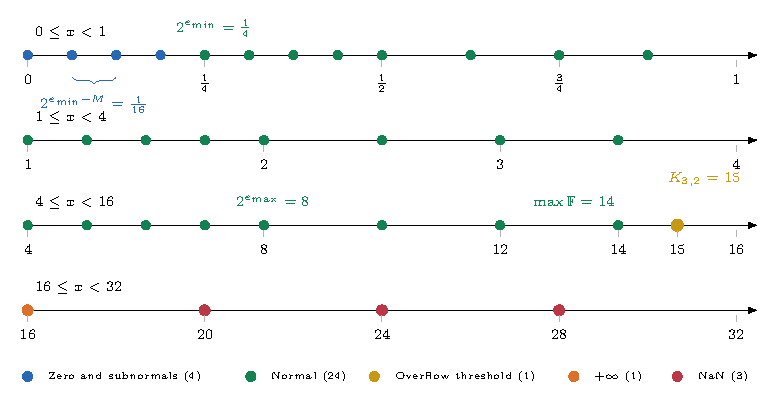
\includegraphics[width=0.98\linewidth]{Figures/FloatingPointSystemE3M2.pdf}
  \caption{The nonnegative $(E,M)=(3,2)$ format: 24 normal values,
  zero and three subnormals, one infinity code, and three NaN codes,
  together with the nonrepresentable threshold $K_{3,2}=15$.
  The last strip arranges special codes by their bit-pattern slots,
  not by real values; $F_{\max}=14$.}
  \label{fig:fp-E3M2}
\end{figure}


\begin{definition}[Rounding]
Let
\[
 F_{\max}=(2-2^{-M})2^{b_E},\qquad
 K_{E,M}=(2-2^{-M-1})2^{b_E}.
\]
Here $F_{\max}$ is the largest finite floating-point value and
$K_{E,M}$ is the positive overflow threshold. The
\emph{round-to-nearest, ties-to-even} map
$\rnd_{E,M}\colon\R\to\overline{\mathbb F}_{E,M}$ is defined by
\[
\rnd_{E,M}(x)=
\begin{cases}
 -\infty,&x\le-K_{E,M},\\
 \displaystyle\operatorname*{arg\,min}_{y\in\mathbb F_{E,M}}|x-y|,
 &|x|<K_{E,M},\\
 +\infty,&x\ge K_{E,M}.
\end{cases}
\]
If two finite values minimize the distance, choose the one whose least
significant stored significand bit is even. In particular, halfway cases
near $0$ round to $0$; the chosen value always exists and is unique.
\end{definition}

\begin{proposition}[Monotonicity of Rounding]
For $x,y\in\R$,
\[
 x\le y\quad\Longrightarrow\quad
 \rnd_{E,M}(x)\le\rnd_{E,M}(y),
\]
with the usual order on $\R\cup\{-\infty,+\infty\}$.
\end{proposition}
Strict monotonicity does not hold: distinct real numbers can round
to the same floating-point value.

\begin{definition}[Floating-Point Operations]
For $a,b,c\in\mathbb F_{E,M}$, define rounded arithmetic by
\[
\begin{aligned}
 a\oplus b&=\rnd_{E,M}(a+b),&
 a\ominus b&=\rnd_{E,M}(a-b),\\
 a\otimes b&=\rnd_{E,M}(ab),&
 a\odiv b&=\rnd_{E,M}(a/b)\quad(b\ne0).
\end{aligned}
\]
The secondary notations are $\odot$ for multiplication and $\oslash$
for division. \emph{Fused multiply-add} performs only one rounding:
\[
 \fma(a,b,c)=\rnd_{E,M}(ab+c).
\]
These operations have values in $\overline{\mathbb F}_{E,M}$;
operations involving infinities, NaN, or signed-zero bit patterns are
outside the present finite-input definitions.
\end{definition}

\begin{remark}[Algebraic Properties]
Rounded addition and multiplication are commutative, with identities
$0$ and $1$, but generally neither associative nor distributive. For
$(E,M)=(3,2)$, ties-to-even gives
\[
\begin{aligned}
 (1\oplus\tfrac18)\oplus(-1)&=0
     \ne\tfrac18=1\oplus(\tfrac18\oplus(-1)),\\
 2\otimes(\tfrac34\otimes\tfrac18)&=\tfrac14
     \ne\tfrac3{16}=(2\otimes\tfrac34)\otimes\tfrac18,\\
 3\otimes(1\oplus\tfrac32)&=8
     \ne7=(3\otimes1)\oplus(3\otimes\tfrac32).
\end{aligned}
\]
Every $a\in\mathbb F_{E,M}$ has the unique additive inverse $-a$,
since $a\oplus b=0\iff b=-a$ (all finite values are integer
multiples of the smallest subnormal spacing). Multiplicative inverses
need not exist or be unique. In the same format,
\[
 \tfrac32\otimes\tfrac58=1=\tfrac32\otimes\tfrac34,
 \qquad \tfrac1{16}\otimes b\ne1\quad(b\in\mathbb F_{3,2}).
\]
Moreover, rounded operations may overflow to $\pm\infty$, outside
$\mathbb F_{E,M}$; hence they do not form a field.
\end{remark}

\Needspace{8\baselineskip}
